\documentclass[11pt,letterpaper]{article}
% vim: nospell

% \usepackage{fancyhdr} % fancy headers
\usepackage{geometry} % page geometry package
% \usepackage{sectsty}  % change the size of sections
% \usepackage{amsmath} % equations in \align
% \usepackage{enumitem} % fancy enumerators
% \usepackage[linesnumbered,lined,ruled,commentsnumbered,shortend]{algorithm2e} % pseudocode
% \usepackage{comment}
\usepackage{hyperref} % hyperlinks
% \usepackage{graphicx} % including images
% \usepackage{fancyvrb} % sophisticated verbatim text
% \usepackage[dvipsnames]{xcolor}   % pretty colours

%
% geometry
%
% \hoffset    = -0.5in
% \voffset    = -0.25in
% \textwidth  = 7in
% \textheight = 8.5in
\headheight = 26pt

%
% fancyhdr
%
%\pagestyle{fancy}

%
% secsty
%
%\sectionfont{\fontsize{12}{15}\selectfont}

%
% fancyvrb
%
%\RecustomVerbatimCommand{\VerbatimInput}{VerbatimInput}%
%{fontsize=\footnotesize,
%  %
%  frame=lines, % top and bottom rule
%  framesep=1em, % separation between frame and text
%  rulecolor=\color{Gray},
%  %
%  % label=\fbox{\color{Black}data.txt},
%  label=\fbox{\color{Black}},
%  labelposition=topline
%  % commentchar=# % ignore lines starting with commentchar
%}


\begin{document}

\section{Basic Information}
$\ $

\begin{tabular}{ll}
	Name & Peter Olson \\
	Email & p.olson@wustl.edu \\
	Student ID & 441666 \\
	Repository & \href{https://github.com/BackToTheDrawingBoard/cse557-fl18-information-visualization-final-project}{GitHub repository link}
\end{tabular}


\section{Background and Motivation}
During my junior year, I took Dr. Anupam Basu's Introduction to Digital
Humanities course, in which we discussed topic models.  In our class, we
explored a tool called
\href{http://vep.cs.wisc.edu/serendip/}{Serendip}, which visualizes
topics as a matrix of relationships between texts in the corpora and
topics.  Then, this semester, I took Dr. Neumann's Analysis of Network
Data class, and it occurred to me that Serendip's matrix presentation of
the topic model is visually similar to an adjacency matrix.

I want to take a distinctly different approach than Serendip, though.
While Serendip focuses on drilling down into specific relationships and
presenting a large volume of information at once, I want to focus more
on exploring the topic-story relationship in a more approachable,
intuitive manner.

\section{Project Objectives}
I would like to build an interface that allows for the creation and
exploration of simple topic models, with a focus on drawing out the
abstract relationship between a topic and a set of stories.  I'd like to
emphasize exploring the relationship as a two-way street, not just from
the perspective of looking at the topic model of individual stories.

\section{Data}
Because topic modelling is such a versatile tool, I can create corpora
of almost any source of textual data.  Hypothetical sources include the
lyrics of popular songs, well-known novels, plays, or even technical
documents, such as white-papers and specifications.

At least initially, I'm planning on following in the foot steps of
Introduction to Digital Humanities and creating a corpus of books from
\href{https://www.gutenberg.org/}{Project Gutenberg}.

\section{Data Processing}
As far as manual cleanup of the corpus itself, I'm going to need to
remove any extraneous text, so that the source files are only the raw
text documents for the corpus.  In the case of documents from Project
Gutenberg, I'll need to remove the header and footer that Project
Gutenberg attaches. Other than the header and footer, the text files
available there are relatively free of markup and extraneous
information.

I'm planning to do the topic model generation in the browser.  There are
several Javascript libraries (such as
\href{https://mimno.infosci.cornell.edu/jsLDA/}{jsLDA}) that implement
topic modelling without relying on running a server.  I also have a
rudimentary implementation of topic model generation that I could use,
but it's definitely inferior to libraries developed by actual
machine-learning developers.  I'm just a computer engineer.

\section{Visualization Design}
% How will you display your data? Provide some general ideas that you
% have for the visualization design. Create three alternative designs
% for your visualization. Create one final design that incorporates the
% best of your three designs. Describe your designs and justify your
% choices of visual encodings. You use the Five Design Sheet
% Methodology.

The center of my visualization is going to be a force-network
visualization of the topic-story relationships.  Accompanying this
representation, I'm going to also have accompanying histogram views of
the occurrences of topics in individual stories, as well as a pane that
simply displays detailed information about a story or topic if selected
in the force-network.

The thesis of my design is that I want to push that the relationship
between topics and documents isn't necessarily hierarchical.  That is to
say that topics aren't exclusively observations on documents, and
documents aren't solely representations of topics.  By representing both
topics and documents as nodes in a force-network, they're given
explicitly equal roles in the way that the network is constructed.  I'm
toying around with the idea of having the ability to switch which class
of node generates force within the graph, so that each class of node can
be positioned in the graph in relation to the other.

My design very much benefits from related work done in Serendip and
SerendipSlim, as those tools act as useful foils for my visualization.
I explicitly want to detach from the hyper-analytical approach that
Serendip takes.  Serendip is mostly interested in analyzing the topic
model itself, whereas I am more focused on exploring the relationships
created between stories and topics.

\section{Must-Have Features}
\begin{itemize}
	\item Topic-Model generation
	\item Presentation of resulting topics
	\item Network graph of topic-story relationships
	\item Alternative content-view for presenting per-story topic 
		breakdown
	\item A "details" pane that exposes more information about a topic or
		story when selected.
\end{itemize}

\section{Optional Features}
\begin{itemize}
	\item Customization of topic-model parameters
	\item Coding the weight of the relationship strength into the link
		between stories and topics
	\item Some means of filtering the documents displayed
	\item Preset configurations for the network
	\item Lasso selection of nodes in the network display
\end{itemize}

\section{Project Schedule}

\begin{tabular}{|r|c|l|}
	\hline
	                          &  Nov. 9th & Topic-model debug output \\
														&           & Dummy network with working forces\\\hline
	              Milestone I & Nov. 13th & Card for topics on the sidebar \\\hline
							 Milestone II & Nov. 27th & Filtering topics \\
														&           & Link network with topics \\\hline
					 In-Class Studies & Nov. 29th & \\\hline
	                          &  Dec. 7th & Outline presentation \\
														&           & Process book \\\hline
	                          & Dec. 14th & Finish presentation \\
														&           & Glitz and color \\\hline
	Submission + Presentation & Dec. 19th & \\\hline
\end{tabular}

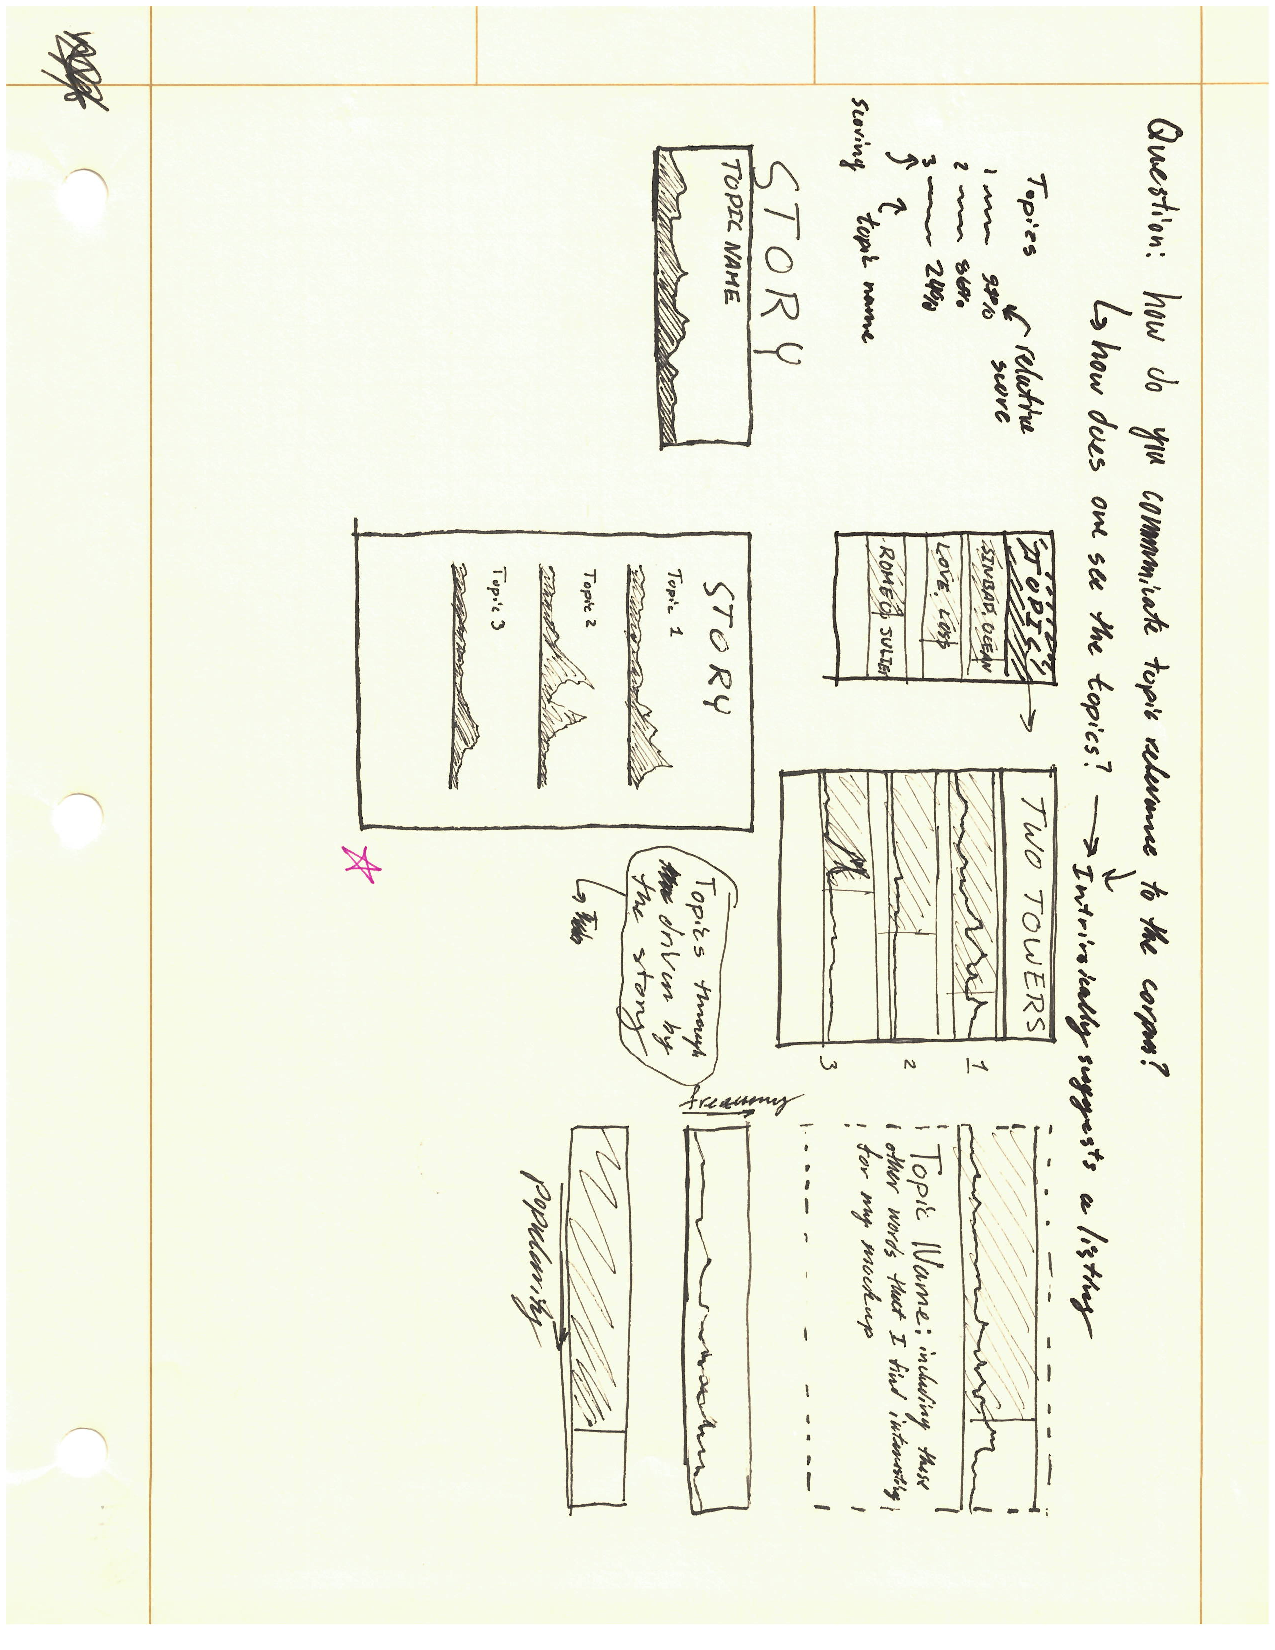
\includepdf[pages=-]{sketches.pdf}
\end{document}
